\chapter{Pulitzer Prize-Winner Explains His Writing Process --- Richard Powers}

This lecture opens twice. First comes the compressed maxim: push a character to the wall and drama appears. Then the conversation restarts more patiently, naming its terrain --- drama, conflict, voice, dialogue --- and rebuilding the claim from ordinary social life outward. That double opening matters. We are given the answer before we are shown the machinery. Our task in these notes is to preserve that rhythm: pressure first, then character, then widening scales of conflict, and only after that the granular craft of words, syntax, tension, and revision.

\section{Character, Pressure, and the Three Levels of Drama}

Powers begins where a dramatist should begin: not with plot machinery, but with a person under strain. Character, he says, is complex, and we do not really see that complexity until circumstances force a choice. This is the cold-open thesis, and it can be written in its most compact form as
\begin{equation}
\text{character} \Rightarrow \text{drama}.
\end{equation}
We should hear this carefully. The claim is not that drama is pasted onto character from the outside. The claim is that character becomes legible only when the pressure is high enough. If nothing is at stake, we may get traits, surfaces, and manner, but not necessity.

The lecture then performs one of its favorite escalations. We begin with person against self and person against person. Is that it? No. There is a third scale. Powers names the full hierarchy as
\begin{equation}
\text{person vs self},\qquad \text{person vs person},\qquad \text{person vs world}.
\end{equation}
The first is interior collision. The second is social and political collision. The third is the collision between a human project and the larger world within which that project must live.

After the cold open, the interview restarts in a different register and gives us the lecture's first major motivation: character is not an exotic literary invention. We are already doing it all the time. Human beings survive socially by inferring hidden motives, old grudges, unspoken nostalgias, and alternate futures in one another. We are, Powers says, all novelists in our own lives. Fiction refines a faculty that ordinary life has already trained.

That is why the lecture next turns to living fictional examples rather than abstractions. Powers speaks of the protagonists in \emph{Playground} --- Todd Keen and Rafael --- as figures through whom he could let unfinished material from his own past collide in dramatized form. The point is not autobiography alone. The point is that character, once made active enough, tends naturally toward conflict. Friendship, rivalry, distrust, class difference, mutual need: these are not decorations around persons. They are the local forms through which drama begins to grow.

\subsection{Question \& Answer}

\paragraph{Question.} Where does drama actually come from?

\paragraph{Answer.} It comes from collision made unavoidable. A character is pushed to the wall, two values become incompatible, two people need different things, or a human project runs into the larger world. ``Push them to the wall'' is not merely advice about intensity; it is the lecture's first real method.

\section{The Onion of Character: Traits, Mannerisms, and Core Inner Values}

Once Powers has persuaded us that character is already latent in everyday life, he turns from intuition to procedure. Here the lecture becomes explicitly pedagogical and leans on Stanislavski. The actor, and likewise the novelist, must inhabit a person who is not identical with the self. One does this not by imitation alone, but by locating something inward and fundamental that one can enter.

His teaching image is the onion. On the outside are traits; beneath them are mannerisms; beneath these lie core inner values. In compact form:
\begin{equation}
\text{core inner values} \to \text{mannerisms} \to \text{traits}.
\end{equation}

\begin{figure}[h]
\centering
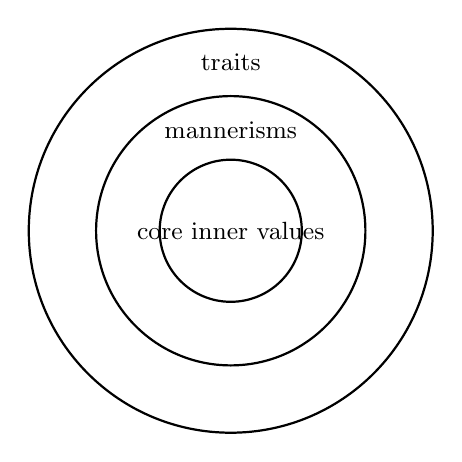
\begin{tikzpicture}[scale=0.95]
\draw[thick] (0,0) circle (2.7);
\draw[thick] (0,0) circle (1.8);
\draw[thick] (0,0) circle (0.95);
\node at (0,2.25) {\small traits};
\node at (0,1.35) {\small mannerisms};
\node at (0,0) {\small core inner values};
\end{tikzpicture}
\caption{Transcript-based schematic reconstruction of Powers's ``onion'' model of character.}
\end{figure}

Traits are the outer shell: the visible or performative details by which a reader first takes hold of a person. Mannerisms sit below that shell: repeated habits of challenge, soothing, evasion, display, or control. Core inner values lie deeper still: honesty, fidelity, perseverance, freedom, equality, attentiveness, complicity. These values are not interchangeable ornaments. They are the inward commitments a character is trying to preserve in the world.

Powers is careful not to make the onion too mechanical. The arrows are not one-to-one. Multiple values may underwrite the same mannerism, and multiple mannerisms may support the same visible trait. That is why characterization is not solved by inventory. It is solved by coherence. Outer behavior must hide and reveal at the same time.

The Nemo example in the lecture is useful precisely because it makes this structure teachable. A father's overprotectiveness is not merely a trait. It is a visible pattern issuing from deeper commitments: fear, love, protectiveness, the refusal to risk loss again. Once we see that, the surface becomes dynamic rather than merely descriptive.

\paragraph{Worked derivation.} Powers's procedure for turning description into drama can be written as a short chain:
\begin{enumerate}
\item Begin with a visible trait.
\item Ask what mannerism or recurring behavior produces that trait.
\item Ask what core inner value could underwrite that mannerism.
\item Add a second value the character also refuses to surrender.
\item Construct a situation in which both values cannot be preserved.
\item The forced loss produces interior drama.
\end{enumerate}

This is why the lecture's signature example is so strong:
\begin{equation}
\text{honesty} + \text{fidelity} + \text{forced choice} \Rightarrow \text{interior drama}.
\end{equation}
A friend has done something wrong. Shall we tell the truth and betray the friend, or remain loyal and betray the truth? The story does not begin with the labels alone. It begins when the labels can no longer coexist.

\subsection{Question \& Answer}

\paragraph{Question.} How do we turn a person into a dramatic character rather than a mere description?

\paragraph{Answer.} We move downward before we move outward. We infer values beneath mannerisms and mannerisms beneath traits. Then we make those values collide. Description becomes character only when something inward must be chosen and something inward must be lost.

\section{Beyond the Human World: Ecological and Metaphysical Drama}

At this point the lecture widens its scale again. The move is characteristic of Powers: person against self, person against person --- is that enough? No. Human beings do not merely collide with other human beings. They also collide with the terms set by a world that is larger than they are.

He names the widening like this:
\begin{equation}
\text{psychological} \to \text{sociological/political} \to \text{environmental/metaphysical}.
\end{equation}
The first two kinds of drama have been dominant in much modern fiction. The third, Powers argues, was often thinned out or neglected. Literary fiction became exceedingly adept at inner life and social life while too often treating human beings as though they were autonomous from everything else.

This is why the lecture spends real time on literary history. The old ``man against nature'' story comes to seem quaint, even though myth, epic, frontier fiction, \emph{Moby-Dick}, science fiction, and fantasy never really lost it. The dip, for Powers, was not the disappearance of the third drama everywhere; it was the narrowing of what counted as respectable literary seriousness. For a long stretch, serious fiction could behave as if human beings had already won the struggle against the nonhuman world. Ecological crisis has ended that illusion. The third drama has returned because the world has returned as an active term in the equation.

We can state the three scales of conflict and their widening field in a single visual line:
\begin{equation}
\text{person vs self} \Rightarrow \text{person vs person} \Rightarrow \text{person vs world}.
\end{equation}
The arrows here do not mean that the later scale replaces the earlier one. They mean that the later scale contains and enlarges it.

This is where Powers turns to trees, childhood animism, and older literatures. The move is easy to misunderstand if we flatten it into ``environmental themes.'' That would be too weak. His stronger claim is that attention to the nonhuman world is another route into interior drama. A child sees aliveness where adults see only wood. Oral literatures knew that we cannot understand human beings except in conversation with what we are not. Hence the striking sentence in the lecture: to look at the nonhuman world is also to understand interior drama.

Powers's fusion of science and animism follows directly. We must know the world as science knows it and as an animist child knows it. These are not enemy programs. They are two forms of access to a reality that is richer than either one alone can hold.

\subsection{Question \& Answer}

\paragraph{Question.} Why must stories move beyond the human if they are to capture the full scale of drama?

\paragraph{Answer.} Because human life is not self-sealed. Our values and projects take shape inside a larger living world that may resist, ignore, or transform them. If fiction omits that dimension, it does not become purer; it becomes narrower.

\section{Why Fiction Moves Us: Story, Affect, and Value Change}

Having widened the scale of story, Powers turns to the question of force. Why can fiction matter at all? The immediate motivation in the lecture is concrete. David reads passages from \emph{The Overstory} aloud and feels that the novel is doing something beyond information. Powers names the difference with great clarity:
\begin{equation}
\text{apprehension of fact} \neq \text{shift in values}.
\end{equation}
We may learn something intellectually and yet remain unchanged in what we care about. Facts can be grasped without becoming commitments.

The novel works by another route:
\begin{equation}
\text{story} \Rightarrow \text{affect} \Rightarrow \text{identification} \Rightarrow \text{movement of the reader}.
\end{equation}
This is why his etymological aside about emotion matters. Emotion is not merely a feeling we possess; it is something that moves through us and moves us onward. A story does not merely instruct. It re-situates the reader inside another perspective.

The lecture makes this concrete through a familiar kind of psychology experiment. The details matter, because Powers is not making a mystical claim; he is describing a mechanism.

\paragraph{Worked example.} The helping-behavior experiment unfolds as follows:
\begin{enumerate}
\item Different groups of subjects are asked to read different texts under the guise of a comprehension exercise.
\item One group reads neutral material; another reads non-affective data; another reads a fictional passage capable of producing feeling and identification.
\item After answering comprehension questions, the subjects leave the room.
\item In the hallway, a confederate drops pencils or spills carried materials.
\item The group that has just read the moving story is more likely to stop and help.
\end{enumerate}
The inference is not that fiction permanently saves us. The inference is more modest and more interesting: identification baseline-shifts the reader, even if only for a moment, into greater sympathy and responsiveness.

This is the strongest answer the lecture gives to the old rivalry between argument and narrative. Bare argument may secure assent. Story may change what a reader is prepared to do. That is why Powers later compresses the point into a hard maxim of his own: the best arguments do not necessarily change a mind; a good story may.

\subsection{Question \& Answer}

\paragraph{Question.} Why can a story move a reader when an argument cannot?

\paragraph{Answer.} Because story changes the route of entry. Argument addresses belief directly. Story recruits affect, and affect recruits identification. Once the reader asks, ``Who would I be if I were that person?'', the resulting change is no longer merely conceptual. It becomes active.

\section{Voice from Below: Register, Diction, Syntax, and Predication}

Only now does the lecture descend to its nuts and bolts. That order is essential. Powers does not begin with craft trivia and hope the stakes will arrive later. He first tells us what fiction does; only then does he ask how its machinery works.

He introduces this descent with one of the lecture's strongest images: a novel is a sled pulled by many dogs in harness. Language is one dog, character another, drama another, form and structure others still. The problem is not to choose one and despise the rest. The problem is to get them all pulling in the same direction.

The causal spine is therefore two-step:
\begin{equation}
\text{voice} \Rightarrow \text{character},\qquad
\text{character} \Rightarrow \text{drama}.
\end{equation}
If we allow ourselves a fuller transcript-based reconstruction of the downward chain, we get
\begin{equation}
\text{diction/register/syntax} \Rightarrow \text{voice} \Rightarrow \text{character} \Rightarrow \text{drama} \Rightarrow \text{form}.
\end{equation}

\begin{figure}[h]
\centering
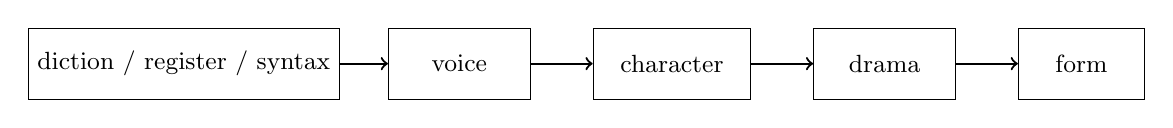
\begin{tikzpicture}[x=1cm,y=1cm]
\node[draw, minimum width=2.7cm, minimum height=0.9cm] (a) at (0,0) {\small diction / register / syntax};
\node[draw, minimum width=1.8cm, minimum height=0.9cm] (b) at (3.5,0) {\small voice};
\node[draw, minimum width=2cm, minimum height=0.9cm] (c) at (6.2,0) {\small character};
\node[draw, minimum width=1.8cm, minimum height=0.9cm] (d) at (8.9,0) {\small drama};
\node[draw, minimum width=1.6cm, minimum height=0.9cm] (e) at (11.4,0) {\small form};
\draw[->, thick] (a) -- (b);
\draw[->, thick] (b) -- (c);
\draw[->, thick] (c) -- (d);
\draw[->, thick] (d) -- (e);
\end{tikzpicture}
\caption{Transcript-based schematic reconstruction of the lecture's downward craft chain.}
\end{figure}

We should notice the sequence. Form is not the top-level shell imposed from above. It emerges from decisions made at lower levels. That is one of the lecture's most important structural claims.

At the lowest level, Powers begins with register. How can we say the same thing in multiple ways? ``Hand me that.'' ``Give me that.'' ``Would you please pass that?'' A mere ``yo'' with a gesture. Each performs the same basic request, but each also broadcasts class, intimacy, authority, distance, ease, aggression, or deference. Voice is already present at the word level.

English gives the writer another lever: its historical bilingualism. Anglo-Saxon and Latinate vocabularies do not merely offer synonyms; they offer shifts in color and social register. ``House'' and ``mansion,'' ``freedom'' and ``liberty,'' carry different historical and socioeconomic freight. Once a writer learns to hear that freight, diction becomes a form of character construction.

But diction is only the beginning. Powers wants a usable grammar for writers, not a return to hated school exercises. So he reduces the sentence to its kernel.

\begin{definition}
By \emph{predication} Powers means the main subject together with the main verb. This is the sentence's central act.
\end{definition}

In compact notation,
\begin{equation}
\text{predication} = \text{main subject} + \text{main verb}.
\end{equation}
Once we hear that kernel, Powers says, we can begin to place it differently and thereby change the reader's mental state. His three sentence classes may be written, cautiously, as
\begin{equation}
SV\cdots,\qquad \cdots SV,\qquad S\cdots V.
\end{equation}
The notation here is editorially compressed, but the first two patterns are strongly supported by the lecture's examples.

\paragraph{Worked example.} The first two classes can be anchored directly:
\begin{align}
\text{He pointed the gun at his friend.} &\sim SV\cdots,\\
\text{Way back across the yard, near the fence, where a tiny brook ran, she hid.} &\sim \cdots SV.
\end{align}
In the first, the kernel arrives immediately. The action shocks us at the front of the sentence, and the rest trails after as consequence. In the second, the modifiers delay the kernel. The reader waits. When ``she hid'' finally arrives, the sentence has hidden her grammatically before the scene reveals her physically.

The third form,
\[
S\cdots V,
\]
must be handled more cautiously. Powers describes it clearly --- split subject from verb, place material in the middle, create suspense, comedy, or a key change --- but he does not exemplify it as fully. What matters for us is the larger principle: sentence shape is not neutral packaging. Syntax itself can participate in the emotional state being represented.

\subsection{Question \& Answer}

\paragraph{Question.} What drives voice if voice drives character?

\paragraph{Answer.} Voice is driven from below. Word choice fixes register; register and diction combine with syntax, cadence, and pacing; those choices give us a speaking presence; and from that presence we infer a character. Voice is therefore not a mystery hovering above the page. It is the audible result of lower-level decisions.

\section{Description, Expectation, and Revision}

Now the lecture does something it repeatedly does well: it stops speaking in formulas and lets a single sentence carry the proof. Powers is asked about description, and he answers not with a general rule but with a line: ``Each child's tree has its own excellence.'' Why does that sentence work? Why does it not collapse into ornament?

First, because the description that follows is doing exact work. The ash, walnut, maple, elm, and ironwood are being made distinct rather than generally picturesque. Description here is classificatory and sensuous at once. Second, because the line contains a small registral and rhythmic surprise. ``Excellence'' is not the obvious word with which to end a sentence about a tree. That end-word matters.

Powers's explanation implies a reader-expectation model. If we allow ourselves a compact editorial shorthand, we may write it as
\begin{equation}
P(w_{n+1}\mid w_1,\dots,w_n),
\end{equation}
not as lecture notation, but as a compressed way of stating his claim that we are always silently forecasting what comes next. The beginning and the end of the sentence are especially charged positions because expectation is high there.

The mechanism may be written schematically as
\begin{equation}
\text{expected ending} \Rightarrow \text{surprising but apt ending} \Rightarrow \text{local increase in tension}.
\end{equation}
The surprise need not be violent. In good prose it is often slight, but slight is enough. ``Excellence'' arrives where a flatter end-word might have been more predictable, and the sentence changes color in its last instant.

\paragraph{Worked example.} The lecture's logic of surprise is simple:
\begin{enumerate}
\item A sentence opening establishes rhythm and semantic expectation.
\item The reader's ear forecasts a likely continuation.
\item A less likely but still exact end-word appears.
\item The sentence closes in a new tonal key.
\item That tonal shift raises tension slightly and keeps the line alive.
\end{enumerate}

The catalogues that follow in this section of the lecture deepen the point. ``The ironwood's fluted muscle'' is not merely vivid. It is a controlled invitation to animism. The trunk is made bodily without becoming crudely sentimental. Likewise, ``the pencil dreams of boys'' first feels odd and then, as the catalogue expands, places the reader inside a recognizably childish imaginative state. Description succeeds not by saying more and more, but by placing the reader in the right psychic relation to what is seen.

This leads Powers to revision, and here the lecture becomes especially humane. The first draft is permitted to show its effort. One may have to overstate an intention in order later to hide the footwork. Revision is not the bureaucratic cleanup after writing; it is writing continued under finer perception.

Powers even calls this ``lesson number one of craft.'' When he hears his own earlier prose, he wants a red pen. That is not a defect in the process. It is the process. The writer is a moving target, the reader is a moving target, the world is a moving target. Therefore there is no final right. Frustration is not merely unpleasant; it is diagnostic. It tells the writer where desire has outstripped execution.

\subsection{Question \& Answer}

\paragraph{Question.} How do we write vividly without sounding overwritten?

\paragraph{Answer.} We first discover the intended effect, even if the draft shows too much effort. Then we revise toward exactness, surprise, and concealment. Vividness does not come from piling on details. It comes from choosing the detail or the word that reorganizes the reader's attention.

\section{Openings, Tension Graphs, Dialogue, and the Writing Life}

From sentence-level expectation the lecture rises back to whole-book form. Openings come first. Powers likes beginnings that act like distant establishing shots in film: cosmic, mythic, or otherwise wide enough to announce the size of the canvas before narrowing toward a local story. The beginning of \emph{The Overstory} and the beginning of \emph{Playground} both work this way. They do not merely begin the plot; they declare scale.

This is why Powers loves opening lines in other writers as well. A first line may contain the whole book in miniature, not because the reader can decode it immediately, but because the conflicts are already compressed inside it. The opening is therefore not external packaging. It is an early act of form.

That leads directly to the lecture's most explicit theory of long-form structure. Once we are dealing with collision, the primary formal variable is tension.

\begin{definition}
Tension is the realization, first within the protagonists and then in the reader, that the stakes are going up.
\end{definition}

In the lecture Powers first teaches a four-part graph and only then adds the aftermath. The initial structure is
\begin{equation}
\text{hook} \to \text{exposition} \to \text{rising action} \to \text{climax},
\end{equation}
and the extended version is
\begin{equation}
\text{hook} \to \text{exposition} \to \text{rising action} \to \text{climax} \to \text{denouement}.
\end{equation}
The engine inside the middle is recursive:
\begin{equation}
\text{solve local instability} \Rightarrow \text{larger instability}.
\end{equation}
This is what keeps a long narrative from flattening into repetition.

A negative example in the lecture makes the rule obvious. Suppose a prince kills the hardest dragon first, then a somewhat challenging dragon, then the easiest dragon last. The sequence feels wrong at once. Whatever deeper explanation evolutionary psychology might someday give, our narrative sense already knows that stakes must be managed upward, not downward. Yet simple monotonic ascent is not enough either. The shape must be sculpted.

\paragraph{Worked derivation.} Powers's tension graph may be written as a practical sequence:
\begin{enumerate}
\item Begin with a \emph{hook}: tension is raised slightly above rest.
\item Relax into \emph{exposition}: orient the reader, get the players on stage, define the field.
\item Enter \emph{rising action}: expose instabilities already latent in the situation.
\item Let each apparent solution generate a larger instability.
\item Continue until the stakes can no longer be increased.
\item That limit is \emph{climax}.
\item After the climax, release consequence back into the world.
\item That release is \emph{denouement}.
\end{enumerate}

\begin{figure}[h]
\centering
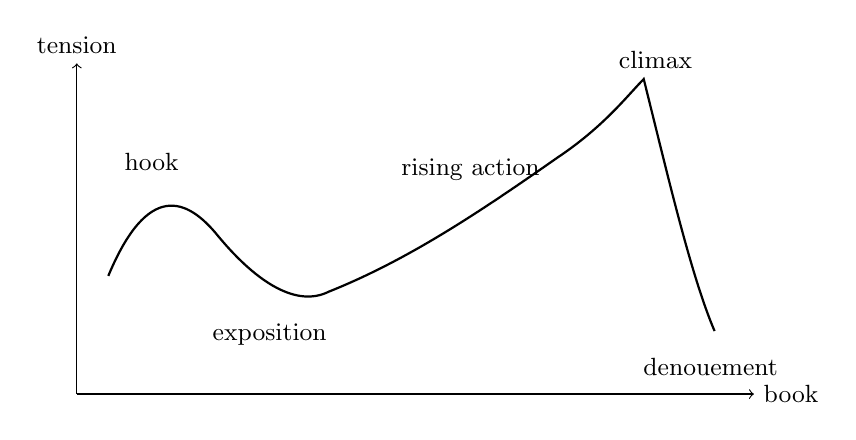
\begin{tikzpicture}[x=1cm,y=1cm]
\draw[->] (0,0) -- (8.6,0) node[right] {\small book};
\draw[->] (0,0) -- (0,4.2) node[above] {\small tension};
\draw[thick] (0.4,1.5)
  .. controls (0.9,2.7) and (1.4,2.5) .. (1.8,2.0)
  .. controls (2.3,1.4) and (2.8,1.1) .. (3.2,1.3)
  .. controls (4.2,1.7) and (5.1,2.3) .. (6.1,3.0)
  .. controls (6.7,3.4) and (7.0,3.8) .. (7.2,4.0)
  .. controls (7.5,2.8) and (7.8,1.5) .. (8.1,0.8);
\node at (0.95,2.95) {\small hook};
\node at (2.45,0.75) {\small exposition};
\node at (5.0,2.85) {\small rising action};
\node at (7.35,4.25) {\small climax};
\node at (8.05,0.35) {\small denouement};
\end{tikzpicture}
\caption{Transcript-based schematic reconstruction of Powers's long-form tension graph.}
\end{figure}

We should also notice Powers's gloss on denouement. It is not merely revelation. It is the loosening or blowing apart of a knot that has been tightened over the course of the book. After climax, the reader needs enough aftermath to understand what those decisive choices will mean in the world.

\subsection{Question \& Answer}

\paragraph{Question.} How does drama generate structure over the length of a whole book?

\paragraph{Answer.} Because the same collisions that animate a scene also determine the book's tension profile. Form is not imposed from outside the drama. It is the large-scale management of rising and falling stakes.

The lecture does not end there. It returns from form to craft in use. Dialogue, Powers says, is not empirically exact speech. If we transcribed a bus conversation word for word and printed it as fiction, it would be nearly unreadable. Good dialogue is stylized. Its realism is conventional, not stenographic. It sounds alive because it knows how to satisfy and bend the reader's expectations about speech at a given historical moment.

That is why Powers insists that dialogue be heard aloud. Readers subvocalize; writers should test the line in the ear. This does not produce only one valid style. Powers admires writers as different as Ann Patchett and Don DeLillo. One may vanish into the naturalness of the speaking character; another may heighten the absurdity of people talking past one another. Both can be true, if the ear holds.

Late in the lecture, another practical principle appears: attention. Powers says that before writing \emph{The Overstory}, the path from his house to his office was simply ``tree, tree, tree.'' During the book it became species: red oak, maple, hornbeam. Deeper still, it became this individual tree, doing something no other nearby tree was doing. Attention increases granularity, and granularity feeds prose. Looking harder is not peripheral to craft. It is one of craft's sources.

The lecture's recurring harness image returns here in another form. A book should not be forced into a choice between head and heart, system and feeling, structure and emotion. The work becomes stronger when these elements support one another and emerge from decisions made lower down.

This brings Powers to solitude and daily practice. Solitude matters, but only as one half of a rhythm. One enters solitude to quiet the world enough for scenes and sentences to gain traction. One leaves solitude to test those products against the world again. A useful late summary is
\begin{equation}
\text{solitude} \to \text{composition} \to \text{return to the world} \to \text{correction}.
\end{equation}
Early in his career the discipline was numerical:
\begin{equation}
1000\ \text{words/day}.
\end{equation}
Later, the accountability changes. The task becomes not merely to extract a quota from the self, but to be in the living world, to check the weather and the calendar, to ask where the day's amazement and instruction are to be found. Then sentences come as a supporting consequence of attention rather than as a purely forced output.

The lecture ends, then, not with a rigid method but with a larger cycle. Writing moves between pressure and replenishment, between form and perception, between inward making and outward correction. That final rhythm is as important as any local tip about sentences.

\section{Summary}

Powers gives us a chain rather than a bag of advice. Character becomes visible under pressure. Pressure yields drama. Drama widens from the inward to the interpersonal and then to the environmental or metaphysical. Fiction matters because information alone does not shift values; story recruits affect and identification. Voice arises from words, register, syntax, and predication. Description works by attention, expectation, and controlled surprise. Revision never truly ends because writer, reader, and world continue to move. On the scale of the whole book, drama becomes form through the management of tension. And on the scale of a writing life, the work proceeds by a repeated exchange between solitude and the living world.